\chapter{Grasping}
Grasping is the activity in which the robot extends its body by attaching an external object to its kinematic chain. This allows the robot to move this object and potentially manipulate it, that is change its shape or pose. Grasping has the interesting, and very confusing, property that its relatively easy in practice, but very difficult in theory. In particular, this chapter is able to describe a variety of strategies that will lead to successful grasps for a wide range of objects, but has difficulties to answer questions such as \emph{What makes a good grasp?} or \emph{How to find good grasps?} in any more depth than by providing simple heuristics.

\section{The theory of grasping}
The theory of grasping is quite involved, with the state of the art comprehensively described in \cite{rimon2019mechanics}, yet has difficulties to mathematically exactly capture the mechanics of grasping mechanisms that are successful in practice. Rather than describing these developments here --- which will be well beyond the scope of this book --- we will briefly describe different approaches to model grasping, and there limitations, to provide an understanding of what the reasons for grasps that work.

\subsection{Friction}\index{Friction}
In its most simple form, grasping requires immobilizing an object, at least agains the forces of gravity, by providing appropriate forces in the opposite direction. Specifically, contact points on a robotic finger, gripper or hand are assumed to exert localized forces, thereby constraining the object sufficiently. By this, fingers act essentially as miniature robotic arms, allowing us to apply the methods and tools from previous chapters~\ref{chap:locomotion}--\ref{chap:forces}.

%% DRAWING OF TWO FINGERS HOLDING AN OBJECT WITH TWO FINGERS AND WITH THREE FINGERS. SHOW COORDINATE SYSTEM.
\begin{figure}
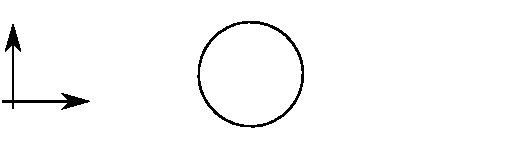
\includegraphics[width=\columnwidth]{figs/idealgrasp}
\caption{Cross-section from above showing an idealized two-finger (left) and three finger (right) gripper holding a cylinder.\label{fig:idealgrasp}.}
\end{figure}

While already very involved for anything but very simple mechanisms, such a model only captures a very small slice of realistic grasps. In any real application, contacts between a gripper and hand are not friction-less. This is the reason a grasp such as shown in Figure~\ref{fig:idealgrasp} actually works. If there were really no friction between the fingers and the object, the object would be ejected from the hand for every grasp that is not exactly aligned with a principal axis of the cylinder in Figure~\ref{ref:fig:idealgrasp}, left. Furthermore, even the three-finger grasp shown in  Figure~\ref{ref:fig:idealgrasp}, right, would \emph{always} fail as there is no force constraining the object from below. Fortunately, the existance of friction makes grasping much easier in practice, yet much harder to describe mathematically.

The reason that the grasps shown in Figure~\ref{fig:idealgrasp} do work in most circumstances is that the normal forces shown have a tangential component that is due to friction and covered by \emph{Coloumb's Friction law,}\index{Coloumb Friction}

which states that the higher the friction coefficient of a material, the more normal force translates into tangential forces that can resist two surfaces from moving against each other:

It is governed by the equation:
\begin{equation}
F_\mathrm{t} \leq \mu F_\mathrm{n}.
\end{equation}

Here $F_\mathrm{t}$  is the force of friction exerted by each surface on the other and $F_\mathrm{n}$ is the normal force. The force $F_\mathrm{t}$ acts in tangential direction of the normal force applied by, e.g., a finger's tip, where $\mu$ is an empirical coefficient of friction.

The friction coefficient $\mu$ is low for glass on glass and high for rubber on wood.  We are therefore interested in designing grippers with high friction coefficients to avoid objects from slipping.

When do objects slip? Lets say we have a fingertip pressing down on a surface in any orientation. There will be a force normal to the surface $F_\mathrm{n}$, which defines the tangential force $F_\mathrm{t}$ in any direction. Sweeping the tangential force around the normal force creates a cone with an opening angle of
\begin{equation}
\alpha=2tan^{-1}\mu,
\end{equation}
see \cite[p. 57]{rimon2019mechanics} for a derivation.
If the net force on the object is not within this cone, the object slips.  This becomes more intuitive when thinking about how different values of $\mu$ affect the shape of this cone. If $\mu$ is high, the cone will be relatively flat, letting the object accept forces from many different directions without slipping. If $\mu$ is low, the cone will be relatively narrow, requiring the force to be normal to the object's surface to prevent slippage.

\begin{figure}
\caption{Left: Coloumb friction relates normal to tangential reaction forces that are required to overcome friction, here shown for rightwards motion. Right: Friction cone for point forces. As long as the force is within the cone cone, the finger will not slip.}
\end{figure}
%% FIGURE SHOWING THE FRICTION CONE

A force applied to a rigid body will exert both a force as well as a torque to the body's center of gravity. This is called a \emph{wrench}\index{Wrench}. If we consider the possible forces that we can apply to a rigid body without having the end-effector slip to form a space (namely the cone described earlier), we can talk about the \emph{grasping wrench space}\index{Grasping wrench space}, which is the corresponding space of all suitable wrenches.

Knowing the relation between normal and tangential reaction forces can help in designing grippers that are more likely to successfully grasp an object than others, as well as when planning suitable grasp for objects with known friction.

%In summary: we can use Coloumb's law of friction to determine the direction of forces that we can apply to a certain contact point without that the object slips. These forces translate into wrenches to the object's center of gravity. A grasp fits a certain task if the wrenches that would fulfill the task can be effectuated without slip. The less force is waisted to overcome slip, the better is the grasp.

\subsection{Multiple contacts and deformation}
In practice, no force will ever be applied at a single point only, but over an area, either due to the size of the finger pad itself or due to the contact area deforming. Even the smallest contact area will allow to not only additional force constraints, but also constraints on torque, thereby adding constraints in additional dimensions and therefore further stabilizing the grasp. This is illustrated in Figure~\ref{fig:contactarea}. Whereas the object can easily pivot around the point of contact in Figure~\ref{fig:contactarea}, left, increasing the area of contact only slighlty constrains the rotational degree of freedom. It is therefore desirable to grasp an object with an as large contact area as possible. (A large contact area will also increase friction.)

\begin{figure}
\caption{From left to right: ideal force exerted via a single point of contact, forces exerted via an area of contact, contact area increasing due to pressure and conforming with the surface.\label{fig:contactarea}}
\end{figure}

A perfectly flat surface has only a single point of contact when grasping a cylinder or sphere. Indeed, using blank metal grippers or fingers is little successful in practice. Instead, rubber pads are used to increase force closure by conforming around the object. As the rubber is flexible, however, the grasp is not completely fixating the object, but it can move within the grasp, which might not be desirable when picking up a nut, e.g., and trying to mount it on a screw.

\subsection{Suction}

A highly capable method for grasping is using suction. Here, a suction cup is pressed against an object, using a vacuum applied by a pump to suck the object against the cup. Instead of exerting forces against the object, which always requires at least one antipodal force (or multiple forces that are distributed such that the object remains in equilibrium), suction only requires one point of contact. The rim of the suction cup provides both friction, to prevent the object to slip, and multiple contact points that further constrain the object beyond the normal force applied by the vacuum. The soft nature of the suction cup provides the ability for the rim to conform to the object, ruling out objects that do not have any flat surfaces. The elasticity of the rim also makes it difficult to further manipulate the object as all forces applied by the robot will need to be transferred via a spring-like elastic material.

\subsection{Non-prehensile manipulation}

\section{Simple grasping mechanisms}

\subsection{1-DoF gripper}
-Example: Utah prosthetic hand
-Strategy: make contact with stiff part until contact is made (touch sensor or wrist force), then close gripper

\subsection{Parallel jaw}
-Most industrial robotic grippers
-Simple kinematics, single motor
-Worm gear drive is slow, range is limited by width of the gripper

\subsection{4-bar linkage}
- Some industrial robotic grippers
- more complex kinematics, single or dual motor
- having two motors can be advantageous, in particular in conjunction with torque control

\subsection{Multi-fingered hands}
- Three finger hand suitable to grasp round object from above
- more difficult to use for other objects
- changing the kinematics from two finger pinching to two-one pinching and three-finger grasps
- more fingers provide additional redundancy, in-hand manipulation

%\section{What is a good grasp?}
%We can also define wrench spaces that suit a specific task, such as picking up an object or opening a door by turning its knob. We can then say that the grasp is ``good'', when the task wrench space is a subset of the grasping wrench space, and will fail otherwise. We can also look at the ratio of forces actually applied to the object and the minimum needed to perform a desired wrench. If this ratio is high, for example, when the robot has to squeeze an object heavily to prevent it from slipping, this grasp is not as good as one, where the ratio is low and all of the force the robot is exerting is actually going into the desired wrench.


\section{How to find good grasps?}

It is usually not possible to find close-form expressions for the grasping wrench space. Instead, one can sample the space of suitable force vectors, e.g., by picking a couple of forces that are on the boundary of the cone's base, and calculate the convex hull over the resulting wrenches.



We are able to determine whether a contact point leads to a good grasp by comparing the grasping wrench spaces that fulfill the task and those that is created by a set of contact points. The question is now how to find good contact points? This is challenging as end-effectors (such as hands) are already quite complicated. A suitable method is therefore to use random sampling, that is bringing the end-effector to random positions, close its fingers around the object, and see what happens when generating wrenches that fulfill the task's requirements.

To close the end-effector's fingers around the object requires collision checking. To see what happens, requires dynamic simulation. In short, collision checking routines model an object using a mesh of triangles that can be generated using CAD tools. These triangles are the leafs of a tree that has a coarse bounding object at the top. This coarse bounding object is then split into smaller and smaller elements. Collision checking can now quickly test whether an object collides at all and then recursively refine the exact triangles that collide and finally find the exact points of collision. Dynamic simulation applies Newtonian mechanics to an object (i.e., forces lead to acceleration of a body) and moves the object at very small time-steps. Detecting a collision usually involves moving the objects one step back and then iteratively approaching them until their proximity exceeds a certain treshold.

\section{Exercises}
\begin{enumerate}
\item Think about at least three mechanisms to realize a parallel jaw gripper. How does the minimum and maximum aperture of the gripper relate to the gripper width for each of these designs?
\item Think about at least three mechanisms to actuate a four-bar linkage. Which of these will keep the payload during power failure?
\item Write code to generate rectangles with random dimensions and orientations. Use a point-in-polygon test to simulate random samples on its surface. Apply principal component analysis to compute the principal axes of the rectangle and compare with ground truth. How does the number of samples affect the accuracy of your estimate?
\end{enumerate}
